
\myChapter{Implementazione di un GA}
Nel seguente capitolo, prendendo spunto da quanto illustrato da Goldberg nel massimizzare una funzione \cite{goldberg1}, mostreremo una semplice implementazione di un GA, partendo dalla costruzione delle strutture dati e dalla applicazione degli algoritmi necessari al suo lavoro; pi\`u nello specifico, utilizzando MatLab ed osservando quanto fatto da Goldberg (seppure con le dovute modifiche), cercheremo di trovare il minimo di una funzione ponendo in mostra le varie fasi di lavoro ed alcuni problemi di implementazione che potrebbero sorgere nell'utilizzo di un GA.
\vspace{3mm}

Ci pare giusto evidenziare il fatto che Matlab implementa gi\`a di default un algoritmo genetico per l'ottimizzazione di funzioni (al tempo stesso ne sono stati sperimentati molti altri \cite{matlab3}) e che ulteriori lavori sono stati eseguiti da diversi esperti del settore e del linguaggio \cite{matlab1} \cite{matlab2}, il nostro compito consisteva nel rendere pi\`u comprensibile l'attuazione di un GA ed il flusso del codice che lo implementa.
\section{Le strutture dati e scelta dei coefficienti}
Gli algoritmi genetici lavorano con stringhe, perci\`o \`e naturale che la popolazione sia un insieme di esse, per l'implementazione del nostro GA di esempio ci baseremo su questo fatto: ogni individuo \`e rappresentato da un array binario, rappresentante i geni, di una dimensione in accordo col problema che affronteremo; la popolazione del GA sar\`a sempre costante (decisa in modo aribitrario) e solamente il miglior cromosoma della precedente generazione sopravviver\`a, unendosi ai nuovi individui prodotti dagli operatori presentati nel capitolo 2.

La funzione che desideriamo minimizzare \`e $$f(x)=(x-7)^2+1$$ nell'intervallo [$0$, $10.23$] con i valori di x equidistanti di $0.01$ fra loro, in modo da avere a disposizione $1024$ possibili punti, l'intervallo \`e stato scelto in modo da semplificare il tutto, dato che per la codifica dei cromosomi dovremmo solamente usare array di dimensione $10$, evitando il sorgere di problemi a causa di codifiche non ammesse; la funzione di fitness corrisponde alla funzione stessa e ci teniamo a precisare che questa \`e una pratica sconsigliata, ma per le finalit\`a dimostrative di questo capitolo risulta essere la scelta migliore. 
I parametri decisi arbitrariamente sono i seguenti:
\begin{itemize}
    \item \textbf{Dimensione della popolazione $30$ costante}, la nuova popolazione sostituir\`a la prima tranne per il cromosoma migliore che rimpiazzer\`a il peggiore fra quelli generati.
    \item\textbf{Coefficiente di crossover 0.75}, un coefficiente di crossover troppo basso implicherebbe un aumento delle iterazioni del ciclo principale; un crossover pari ad 1, invece, permette il minor numero di iterazioni, ma non comporterebbe alcuna sostanziale modifica al comportamento del GA fra iterazione ed iterazione.
    \item \textbf{Coefficiente di mutazione 0.0333}, un coefficiente pari ad 1 capovolgerebbe completamente i geni degli individui ottenuti dal crossover, viceversa (come abbiamo detto al termine del capitolo 2) uno troppo basso non avrebbe alcun effetto di rilievo. 
\end{itemize}
\definecolor{mygreen}{rgb}{0,0.5,0}
\definecolor{mygray}{rgb}{0.5,0.5,0.5}
\definecolor{mymauve}{rgb}{0.58,0,0.82}
\lstdefinestyle{matlab}{
language=Matlab,
numbers=left,
breakatwhitespace=true,
extendedchars=true, 
keepspaces=true,
keywordstyle=\color{blue},
showstringspaces=false,
stringstyle=\color{mymauve},
commentstyle=\color{mygreen}
}
\lstdefinestyle{matlab2}{frame=single}
\lstdefinestyle{matlab3}{emph={  
    switch, case
    },emphstyle={\color{blue}}%
}
Nel codice sottostante viene mostrata l'inizializzazione della funzione, oltre alla definizione dei parametri prima considerati ed il calcolo del fitness della prima generazione.
\begin{lstlisting}[style=matlab, style=matlab2, style=matlab3]
x=[0.00:0.01:10.23]';
n=length(x);
y=zeros(n, 1);
y(1:n)=(x(1:n)-7).^2+1; %funzione da minimizzare

popSize=30; %dimensione della popolazione
pCrossover=0.75; %coefficiente di crossover
pMutation=0.0333; %coefficiente di mutazione
maxGen=500; %generazione massima

%popolazione iniziale generata casualmente
p=fix(x(n).*rand(popSize,1)*100)/100;

%inizializzazione e calcolo fitness inziale
fitness=zeros(popSize, 1);
fitness(1:popSize)=(p(1:popSize)-7).^2+1;
\end{lstlisting}
Dal codice \`e possibile notare che i valori ancora non codificati della popolazione vengono troncati fino ad avere solo due cifre decimali, tutto ci\`o per rendere ancora pi\`u facile l'implementazione dell'esempio che stiamo esaminando; inoltre \`e giusto evidenziare il fatto che  abbiamo omesso le parti in cui avvengono le scritture a video: il codice integrale \`e incluso nell'apposita sezione a fine tesi.
\vspace{3mm}

Prima di andare oltre, premettiamo che ci sono alternative sicuramente migliori sotto ogni punto di vista a quella presentata in questo capitolo, ma ci teniamo a precisare che tenere l'asticella di difficolt\`a ad un livello non decisamente alto aiuta a comprendere meglio i meccanismi che sono stati introdotti nel capitolo precedente.
\section{Le funzioni cardine del programma}
I tre operatori, per via della poca complessit\`a del problema, possono essere implementati direttamente in segmenti di codice, ma prima c'\`e bisogno di illustrare il flusso del programma per comprenderne appieno il funzionamento; il seguente codice mostra la funzione che si occupa della creazione della nuova generazione attraverso gli operatori a noi noti oltre alla codifica ed alla decodifica degli individui.
\begin{lstlisting}[style=matlab, style=matlab2, style=matlab3]
function [newPopulation,fitness]=GAMatlab(pCrossover,
pMutation, population,fitness)
%
% [newPopulation,fitness]=GAMatlab(pCrossover,
% pMutation,population,fitness)
% Genera la nuova popolazione attraverso gli
% operatori fondamentali dei GA
n=length(population);
chromosomes=zeros(n,10); 
newChromosomes=zeros(n,10);
newPopulation=zeros(n, 1);
k=1; %numero individui della nuova generazione
[fitMin,minIndex]=min(fitness); %fitness minimo
for i=1:n
    %codifica
    chromosomes(i, 1:10)=encode(population(i));
end
while k<n+1
    %selezione
    [parent1,chromosomes2,j]=selection(chromosomes,
    fitness);
    fitness2=fitness([1:j-1 j+1:end]);
    parent2=selection(chromosomes2,fitness2);
   
    %crossover
    if (rand(1)<=pCrossover)
        [son1,son2]=crossover(parent1,parent2);
        
        %mutazione
        son1=mutation(pMutation, son1);
        son2=mutation(pMutation, son2);
        
        %aggiunta all'insieme dei nuovi cromosomi
        newChromosomes(k,1:10)=son1;
        newChromosomes(k+1,1:10)=son2;
        k=k+2;
    end
end
for i=1:n
    %decodifica
    newPopulation(i)=decode(newChromosomes(i,1:10));
end
%calcolo del fitness della nuova popolazione
fitness(1:n)=(newPopulation(1:n)-7).^2+1;

%inserisco il miglior individuo della precedente
%generazione al posto del peggiore di quella attuale
[fitMax, maxIndex]=max(fitness);
newPopulation(maxIndex)=population(minIndex);
fitness(maxIndex)=fitMin;
end
\end{lstlisting}
Partiamo dunque dalle funzioni di codifica e decodifica, per poi avere un'introspettiva migliore delle funzioni principali del ciclo; la codifica di un individuo comincia con il prodotto di esso per 100, in modo da rendere il suo valore intero, per poi convertirlo in un array di caratteri binari che rappresenta il suo cromosoma.
Viceversa la funzione di decodifica, preso in input il cromosoma, lo converte nella sua controparte decimale per poi dividerlo per 100, in modo da ottenere sempre e comunque un valore nell'intervallo [$0$, $10.23$].

Si nota subito come il fatto di avere un array binario consenta pi\`u agilmente la lettura e lo scambio di geni fra due cromosomi, ci teniamo a precisare che per ogni problema di ricerca e/o ottimizzazione esistono innumerevoli codifiche possibili, nel caso preso in esame in questo capitolo \`e ovvio che la conversione binaria gioca a nostro favore in quanto ci rende estremamente banale l'implementazione delle successive funzioni, oltre ad essere perfetta per illustrare quanto spiegato nel capitolo precedente.
\vspace{3mm}
%\subsection{}

Passiamo finalmente nel pieno del GA, pi\`u precisamente nella funzione di selezione: nel codice precedente si pu\`o osservare che, come primo passo, viene estratto un cromosoma \textit{parent$1$} oltre alla lista dei cromosomi (da cui \`e eliminato il futuro genitore per evitare che venga selezionato una seconda volta) ed ad un indice indicante la posizione di tale cromosoma nella lista. Tolta la fitness del primo genitore si procede con la selezione del secondo genitore \textit{parent$2$}, i due cromosomi estratti potranno in seguito partecipare al crossover.
\begin{lstlisting}[style=matlab, style=matlab2, style=matlab3]
function [parent,chromosomes2,j]=
selection(chromosomes,fitness)
sumFit=sum(fitness(1:length(fitness))); %somma totale
n=length(chromosomes);
partSumFit=0; %somma parziale
i=1;
randomPoint=rand(1)*sumFit; %punto casuale
while partSumFit<randomPoint && i<n
    partSumFit=partSumFit+fitness(i);
    i=i+1;
end
parent=zeros(1, 10);
parent=chromosomes(i, 1:10);
if nargout>1
    chromosomes2=chromosomes([1:i-1 i+1:end], 1:10);
    j=i;
end
end
\end{lstlisting}
Per la selezione abbiamo scelto di implementare la versione a \textit{roulette}: per far questo ci siamo serviti della somma totale dei valori di idoneit\`a degli individui e dalla somma parziale di essi: per determinare il punto in cui la "freccetta" dovr\`a fermarsi abbiamo costruito un ciclo while che si arresta se e solo se la somma parziale supera un punto deciso casualmente nell'intervallo [$0$, max(Fitness)] oppure se siamo arrivati in fondo alla "roulette". La funzione restituisce dunque il genitore e, nel caso gli argomenti in output fossero pi\`u d'uno, anche la lista dei cromosomi escluso il genitore appena scelto ed il suo indice in essa.
\vspace{3mm}

Successivamente, con una probabilit\`a pari a \textit{pCrossover}, avviene il crossover, implementato nella sua forma a singolo punto.
\begin{lstlisting}[style=matlab, style=matlab2, style=matlab3]
function [son1,son2]=crossover(parent1,parent2)
son1=zeros(1,10); %primo figlio
son2=zeros(1,10); %secondo figlio
crossPoint=randi(9, 1); %punto di crossover
son1(1:crossPoint)=parent1(1:crossPoint);
son1(crossPoint+1:end)=parent2(crossPoint+1:end);
son2(1:crossPoint)=parent2(1:crossPoint);
son2(crossPoint+1:end)=parent1(crossPoint+1:end);
end
\end{lstlisting}
Il codice \`e veramente autoesplicativo: scelto un punto di crossover
\textit{crossPoint} con valore fra 1 la lunghezza del cromosoma meno $1$, lo scambio di geni avviene fra le posizioni [$1$, crossPoint] e [crosspoint+$1$, n] nelle modalit\`a spiegate nell'apposita sottosezione.
\vspace{3mm}

Per concludere l'illustrazione del funzionamento, mostriamo la sezione di sorgente relativa alla mutazione.
\begin{lstlisting}[style=matlab, style=matlab2, style=matlab3]
function mutChromosome=mutation(pMutation,chromosome)
for i=1:length(chromosome)
    if rand(1)<=pMutation
        chromosome(i)=1-chromosome(i);
    end
end
mutChromosome=chromosome;
end
\end{lstlisting}
Come per il crossover, anche il codice della mutazione \`e di facile interpretazione, ogni gene di un cromosoma ha probabilit\`a di invertire il suo allele pari a \textit{pMutation}.
\section{Risultati dell'implementazione}
Come abbiamo potuto osservare, la messa a punto di un GA non risulta essere uno sforzo immenso, per quanto riguarda la sua efficacia useremo questa sezione per vederne i risultati. Grazie alla chiamata \textit{plot} che ci concede Matlab \`e stato possibile costruire il grafico contenente i risultati del lavoro svolto dal GA e, per via della considerevole semplicit\`a del problema preso in esame, siamo sempre stati in grado di trovare il minimo della funzione $(x-7)^2+1$ nell'intervallo [$0$, $10.23$].
\begin{figure}[H]%
    \centering
    %\hfill
    \subfloat[Prima generazione]{{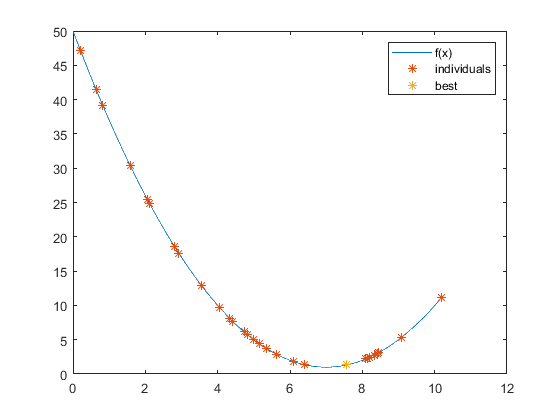
\includegraphics[width=0.5\linewidth]{Images/grafico1.png}}}%
    %\qquad
    %\hfill
    \subfloat[Ultima generazione]{{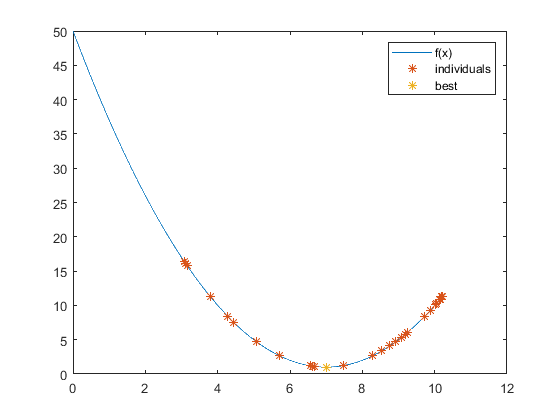
\includegraphics[width=0.5\linewidth]{Images/grafico2.png}}}%
    %\hfill
    \caption{Confronto fra la prima e l'ultima generazione del GA nel problema di minimizzazione presentato}%
    \label{fig:firstfunction}%
\end{figure}
L'immagine soprastante ci conferisce una chiara idea su come si \`e comportato il GA durante l'esecuzione: gli individui col passare delle generazioni tendono ad avvicinarsi al punto di minimo (ovvero 7 nel caso analizzato). L'algoritmo ha concluso le sue operazioni dopo poco meno di 200 iterazioni, delle quali nelle ultime 100 non si sono avuti miglioramenti di fitness, di conseguenza il ciclo \`e stato terminato forzatamente. Altre run del programma hanno portato risultati pi\`u o meno soddisfacenti per quanto concerne la distribuzione degli individui e, per via dell'esigua complessit\`a del problema, la ricerca del minimo \`e sempre terminata con successo.
\section{Considerazioni e problemi ricorrenti}
Il programma in Matlab che abbiamo presentato nell'ultima sezione pu\`o essere modificato in modo tale da minimizzare anche funzioni a due o pi\`u variabili: basterebbe soltanto modificare le funzioni di codifica e decodifica affinch\'e le stringhe che rappresentano i cromosomi contengano e restituiscano informazioni sulle variabili.

Ovviamente \`e possibile cambiare anche i parametri con cui il nostro algoritmo lavora, cos\`i da trovare quelli migliori; il tutto combinato con la possibilit\`a di cambiare anche gli operatori cardine, \`e chiaro come questo sia un indice dell'ampio margine di flessibilit\`a dei GA.
Dunque, a prima vista, il metodo da noi analizzato, ed in generale i GA, sembra essere decisamente efficiente ed efficace, ma ovviamente ad ogni pro corrisponde quasi sempre un contro.

Per mostrare il problema pi\`u ricorrente nei GA ricolleghiamoci alla sezione precedente, in particolare andiamo a testare il nostro programma con un'altra funzione, ossia $$f(x)=\cos{x}*\frac{x}{10}+2$$ sempre nell'intervallo [$0$, $10.23$]; senza riesaminare ogni funzione del nostro algoritmo nei minimi dettagli, mostriamo di seguito l'esito di una qualsiasi run.
\begin{figure}[H]%
    \centering
    %\hfill
    \subfloat[Prima generazione]{{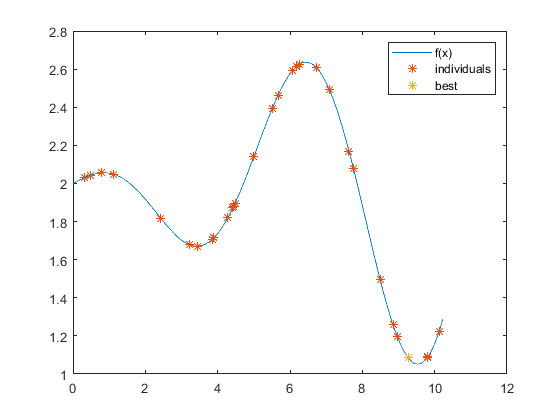
\includegraphics[width=0.5\linewidth]{Images/grafico3.png}}}%
    %\qquad
    %\hfill
    \subfloat[Ultima generazione]{{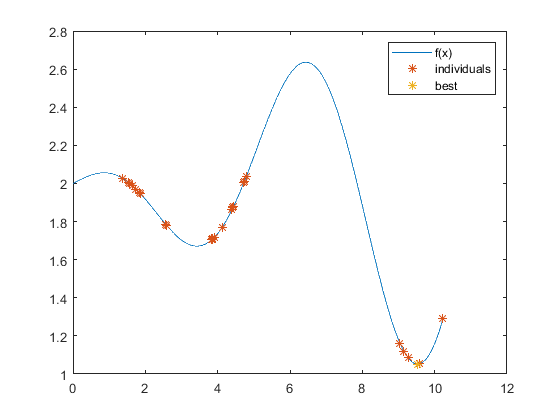
\includegraphics[width=0.5\linewidth]{Images/grafico4.png}}}%
    %\hfill
    \caption{Confronto fra la prima e l'ultima generazione per la nuova funzione considerata}%
    \label{fig:secondfunction}%
\end{figure}
Si nota subito come gli individui si siano aggregati sia nel punto di minimo assoluto (quello che noi volevamo) sia nel punto di minimo relativo, molto spesso in funzioni di questo tipo, ma anche in problemi in cui esistono "falsi ottimi", i GA possono prendere erroneamente la strada sbagliata per poi non riuscire pi\`u a ritrovare la giusta direzione (cosa che \`e successa nel nostro esempio), per ovviare a questi problemi si possono seguire diverse strategie:
\begin{itemize}
    \item Aumentare il coefficiente di mutazione, nella speranza che esso "trascini" gli individui nella direzione voluta.
    \item Ripristinare il GA come se non fosse avvenuta alcuna iterazione, soluzione drastica che non sempre porta risultati migliori di prima.
    \item Rendere "ibrido" il GA: si pensi ad un problema di ordinamento, per iniziare possiamo applicare il nostro GA, nel caso esso non veda progressi di fitness, si attua un algoritmo che sappiamo essere in grado di risolvere il problema (nel nostro caso si potrebbe usare un bubble sort per portare a termine il lavoro richiesto).
\end{itemize}

Potremmo, tramite una metafora, equiparare i GA a degli scalatori ed affermare quanto segue:
\vspace{3mm}

\begin{large}\textit{\textbf{"i GA identificano velocemente le varie vette, ma non sempre riescono a conquistare quella pi\`u alta."}}
\end{large}
\vspace{3mm}

Inoltre, per mostrare come l'approccio illustrato negli ultimi capitoli porta con s\'e alcune lacune, ci teniamo ad aggiungere ulteriori limitazioni nell'uso dei GA:
\begin{itemize}
    \item In quanto alla complessit\`a, non scalano bene all'aumentare di essa: \`e estremamente complicato usare la tecnica dei GA in problemi che possono riguardare il design di automobili o di una casa, per rendere trattabili questi problemi occorre dividerli fino alla pi\`u semplice rappresentazione possibile.
    \item Una determinata soluzione viene ritenuta come la migliore solamente rispetto alla altre, perci\`o il criterio di fermata non \`e chiaro per ogni problema.
    \item Come abbiamo fatto notare poco fa, i GA tendono a convergere verso ottimi locali e non quelli globali.
    \item Operare su insiemi di dati dinamici \`e arduo, siccome pu\`o capitare che i cromosomi convergano presto verso soluzioni non pi\`u valide per dati futuri.
    \item Non possono essere implementati efficaciemente in problemi in cui la funzione di fitness \`e data da una singola risposta booleana (come per i problemi di decisione).
    \item Nel caso vi fossero specifici problemi di ottimazzione od istanze di essi per i quali esistono tecniche risolutive ad hoc, i GA non reggono il confronto per quanto concerne la velocit\`a di convergenza verso la soluzione.
\end{itemize}
Tenendo a mente quanto affermato e mostrato finora, nei prossimi capitoli andremo ad esporre problemi pi\`u complessi rispetto a quello presentato nelle precedenti sezioni, oltre a confrontarli con altri metodi risolutivi pi\`u conosciuti.
\newpage